\documentclass[../DC2017114Bouma.tex]{subfiles}
\begin{document}
\graphicspath{{03_Contribution/img/}}
\renewcommand{\chaptermark}[1]{\markboth{\thechapter.\ #1}{}}
\renewcommand{\sectionmark}[1]{\markright{#1}{}}

\pagestyle{fancyreport}
\cleartooddpage
\pagestyle{fancyreport}
\chapter{Tracking for Hybrid Systems: Ordered State-Input-Triggered Events}\label{ch:order}
In this chapter a control strategy is presented for trajectories of hybrid systems which, due to the introduction of perturbations, experience ordered state-input-triggered events. Such systems are called \textit{nonlinear state-input triggered hybrid systems} (NSITHS). In this chapter ordered state-input-triggered events are considered, which means that the order of events is always known and that there is flow between two events. The perturbations can cause the state trajectory to jump at a different time than the nominal reference trajectory, resulting in \textit{peaking behavior} of the tracking error \cite{Menini2001,Biemond2013}. The work in this chapter is an extension on the work in \cite{Rijnen2017}. First a notion of error is presented, which is used to avoid peaking behavior. After that a first-order approximation of the NSITHS is presented in the form of a \textit{linear time triggered hybrid system} (LTTHS). A proof is given in \cite{Rijnen2017}, which shows that the stability of the LTTHS can be used to asses the local stability of the original NSITHS. Consequentially, conventional stability analysis tools for LTTHS can be used to asses the local stability of te NSITHS. Finally, a short summary of the findings in this chapter is given.
\nomenclature[A]{NSITHS}{Nonlinear State-Input Triggered Hybrid System}%
\nomenclature[A]{LTTHS}{Linear Time Triggered Hybrid System}%

\section{State-input perturbations in trajectories with state-jumps}
This section presents \textit{reference-spreading} (RS) for ordered guard activations. First the tracking problem is presented. The perturbations introduced in the state trajectory cause the state trajectory and reference trajectory to have non-coinciding event-times. This mismatch in event-times results in peaking behavior in the tracking error, meaning that two relatively large jumps can be observed. Using reference-spreading this peaking behavior can be avoided, resulting in a tracking error where only one relatively smaller jump is observed.
\nomenclature[A]{RS}{Reference-Spreading}%

\subsection{Nonlinear state-input triggered hybrid systems}
As presented in Section~\ref{sec:2hyb}, a mechanical system can be described by the hybrid system with impulsive effects framework. Such a system is a nonlinear state-input triggered hybrid system. The NSITHS is now formally defined.

\begin{mydef}[NSITHS]\label{def:3nsiths}
The nonlinear state-input triggered hybrid system is given by
\begin{equation}
\begin{array}{ll}
\dot{\xb}(t,i) =\fb^i(\xb(t,i),\ub(t,i),t),& \xb(t,i),\ub(t,i)\notin D^i\\
\xb(t,i) = \gb^i(\xb(t,i-1),\ub(t,i-1),t),& \xb(t,i-1),\ub(t,i-1)\in D^i
\end{array}\label{eq:3hybimp}
\end{equation}
where $\fb^i$ is a nonlinear Lipschitz continuous function. $D^i$ is a state-input set, with when $\xb(t,i-1),\ub(t,i-1)\in D^i$ a state reinitialization is triggered according to $\xb(t,i) = \gb^i(\xb(t,i-1),\ub(t,i-1),t)$.
\end{mydef} 

The nominal trajectory of an NSITHS is illustrated in Figure~\ref{fig:3perturbedtraj} in red. Now an initial state and input perturbation $\epsilon$ is introduced, which causes the state trajectory $\xb$ to differ from the reference trajectory $\alphab$. The goal is to write a control strategy, such that the perturbed state trajectory $\xb$ will converge to the reference trajectory $\alphab$. Now an initial state-input perturbation $z_0 = \frac{\partial\xb}{\partial\epsilon}$ is introduced, where $\epsilon$ is a scalar perturbation parameter. The initial state $\alphab_0$ and input $\mub_0$ of the reference trajectory $\alphab$ is perturbed, resulting in $\xb_0(\epsilon) = \alphab_0 + \epsilon\zb_0$ and $\ub(t,i,\epsilon) = \mub(t,i) + \epsilon\vb(t,i)$. This generates a trajectory close to the reference trajectory $\alphab$, which is also dependent on the initial state and input perturbation $\epsilon$, i.e., $\xb(t,i,\epsilon)$.
\nomenclature[V]{$\epsilon$}{The scalar perturbation parameter}%
\nomenclature[V]{$(.)_{\epsilon}$}{A variable dependent on the initial perturbation}%
\begin{figure}[h]
\centering
\includegraphics[width=.8\textwidth]{perturbedtraj.eps}\caption{In orange the nominal (unperturbed) and in cyan the perturbed trajectory of a hybrid system with impulsive effects. Due to the perturbation in the cyan trajectory, a mismatch between the perturbed and the nominal event times arises.} \label{fig:3perturbedtraj}
\end{figure}
For the nominal trajectory the state and input are known over the entire time-domain, meaning that the event-times are also known. For the perturbed trajectory this is not the case. Due to the uncertainty in the state and input, there is an uncertainty in the event-times as well. This uncertainty can cause a mismatch between the nominal event times $\tau_1$,$\tau_2$ and the perturbed event times $t_1$,$t_2$. Now we take a closer look at the first event, to illustrate the peaking behavior as a result of a jump mismatch. In Figure~\ref{fig:3peakerror} the state evolution $x$ of the first event is depicted besides the tracking error $||\xb-\alphab||$. Here on can clearly see that a peak arises in the tracking error when the jump times do not coincide. At $t_1$ the state trajectory jumps, while the reference trajectory does not. At $\tau_1$ the reference trajectory jumps as well. This means that in $[t_1,\tau_1]$, a post-event state trajectory is compared to a ante-event reference trajectory, resulting in a large peak in the tracking error. This is undesirable, as it will lead to large and unnecessary actuation forces.

\begin{figure}[h]
\centering
\includegraphics[width=.66\textwidth]{peakerror.eps}\caption{A closer look at the first event of the trajectory in Figure~\ref{fig:3perturbedtraj}. On the left the state-evolution $x$ is depicted and on the right the tracking error $||x-\alphab||$. A clear peak can be noticed in the tracking error as a result from the event-time mismatch.} \label{fig:3peakerror}
\end{figure}

In the next section a solution to the peaking behavior is presented.

\textbf{Existence of guard function assumption (rijnen2017)}
\begin{myass}[Existance of a guard function]
We assume that there exist constants $\varepsilon_\gamma$, and real valued guard function $\gamma(\xb,\ub,t,i)$ which is continuously differentiable with respect to $\xb$, $\ub$, and $t$, for each $i\in \{1,2,...,N\}$, such that
\begin{equation}
\begin{array}{llll}
\gamma(\xb,\ub,t,i) > 0 & &	&(\xb,\ub,t) \in B_{\varepsilon_\gamma}(\alphab(\tau,i),\tau)\cap C^i\\
\gamma(\xb,\ub,t,i) = 0 & &	&(\xb,\ub,t) \in B_{\varepsilon_\gamma}(\alphab(\tau,i),\tau)\cap D^{i+1}\\
\gamma(\xb,\ub,t,i) < 0 & &	&(\xb,\ub,t) \in B_{\varepsilon_\gamma}(\alphab(\tau,i),\tau)\cap (\Rbb^n \times \Rbb^m \times \Rbb)\setminus C^i
\end{array}
\end{equation}
where $B_{\varepsilon_{\gamma}}(\alphab(\tau,i),\tau)$ is a ball with radius $\epsilon_{\gamma}$ around $\alphab(\tau,i)$ with $\tau = \tau^{i+1}$. $C^i$ is the flow set of a trajectory after event $i$ and $D^{i+1}$ is the event set which triggers event $i+1$, which is defined as $\partial C^i$, where $\partial C^i$ represents the boundary of flow set $C^i$.
\end{myass}

\textbf{Locally differentiable jump map assumption (rijnen2017)}.

\begin{myass}[Lipschitz continuity of $\fb$]
We assume that in a neighborhood of the reference trajectory $\alphab$, $\fb$ is Lipschitz with respect to $\xb$ uniformly in $t$ and $i$. I.e., $\exists\varepsilon_{\fb}>0$ and $\exists L$, independent of $t,i$, such that $\forall i$, $||\fb(\ab,t,i) - \fb(\bb,t,i)||<L||a-b||$, $\forall t\in [\tau_i - \varepsilon_{\fb},\tau_i + \varepsilon_{\fb}]$ and $\forall \ab,\bb\in B_{\varepsilon_{\fb}}(\overline{\alphab}(t,i))$, where $B_{\varepsilon_{\fb}}(\overline{\alphab}(t,i))$ is a ball with radius $\epsilon_{\fb}$ around $\overline{\alphab}(t,i))$.
\end{myass}


\nomenclature[V]{$\Delta$}{The linearization of the perturbed event time around zero perturbation}%
\nomenclature[A]{$o(.)$}{Higher order terms}%
\nomenclature[V]{$\Gb_{\zb,i}$}{Positive homogeneous jump gain for the perturbed state direction}%
\nomenclature[V]{$\Gb_{\vb,i}$}{Positive homogeneous jump gain for the perturbed input direction}%
\nomenclature[V]{$D_i(.)$}{The derivative with respect to the $i$th term}%
\subsection{Reference-spreading}
To avoid peaking behavior in the tracking error, in \cite{Saccon2014} a novel notion of error is presented which is named reference spreading in \cite{Rijnen2016}. This control strategy uses reference trajectories which are extended beyond event-times, such that an ante-event state trajectories can always be compared to an ante-event reference trajectory and a post-event state trajectories can always be compared to a post-event reference trajectory. This is illustrated in Figure~\ref{fig:3refspread}, where the reference trajectory segments $\alphab(t,i)$ are all extended resulting in $\overline{\alphab}(t,i)$. The hybrid domain \cite{Goebel2009} of $\alphab$ is defined by segments $I^i_{\alphab} = [\tau_i,\tau_{i+1}]$, which together form the entire domain of $\alphab$ as
\begin{align}
\dom\alphab = \bigcup^N_{i=0}I_{\alphab}^i.
\end{align}
\nomenclature[P]{$I$}{Domain of a segment}%
Similarly the state segments $x(t,i)$ are defined on the domain $I^i_\xb = [t_i,t_{i+1}]$ with the entire domain defined as
\begin{align}
\dom\xb = \bigcup^N_{i=0}I_{\xb}^i.
\end{align}
The domain of the extended reference trajectory segments is extended such that $I_{\xb}^i\subseteq I_{\overline{\alphab}}^i$. \textbf{Define the domain of event times of $\alphab$ (eq 10 of rijnen 2017).}

\begin{figure}[h]
\centering
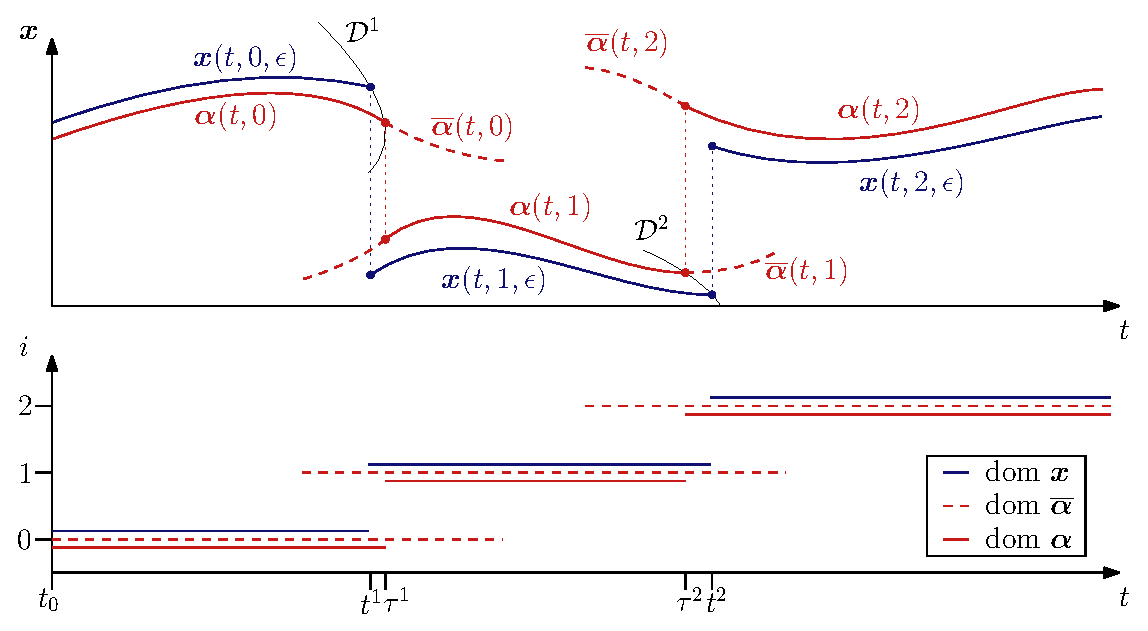
\includegraphics[width=.9\textwidth]{refspreaddom.eps}\caption{An illustration of the nominal reference trajectory (orange) and the perturbed trajectory (cyan), where the nominal reference trajectory is extended such that $\dom x\subseteq\dom \overline{\alpha}$.} \label{fig:3refspread}
\end{figure}

In the lower plot of Figure~\ref{fig:3refspread} the domains of $\xb$, $\alphab$ and $\overline{\alphab}$ are illustrated for each segment. Note that for every segment, $I_{\xb}^i\subseteq I_{\overline{\alphab}}^i$. This means that when the tracking error is defined as $||\xb-\overline{\alphab}||$, we can keep tracking the error $||\xb(t,i)-\overline{\alphab}(t,i)||$ until an event is detected. Even if the event-time $t_i>\tau_i$. When an event is detected, the error  $||\xb(t,i+1)-\overline{\alpha}(t,i+1)||$ can be tracked. Again, because $I_{\xb}^{i+1}\subseteq I_{\overline{\alphab}}^{i+1}$, this is also possible for the case where $t_i<\tau_i$. Using this notion of error leaves only one jump in the tracking error, even under the presence of event-time mismatches. More importantly, the peak in the tracking error is avoided, an ante-event state trajectory will not be compared to a post-event reference trajectory (and vice versa) anymore. In Figure~\ref{fig:3refspreaderrors} the tracking error with and without reference spreading are compared. Here it is clear that the tracking defined using reference spreading does not have the peak which the normal notion of error does have. It also jumps only once at the perturbed event-time $t_1$.
\begin{figure}[h]
\centering
\includegraphics[width=\textwidth]{refspreaderrors.eps}\caption{A close up of the  first event of the reference trajectory, in which the peaking behavior is cleary removed by evaluating the extended reference trajectory.} \label{fig:3refspreaderrors}
\end{figure}

\textbf{Stability definition from Rijnen2017}

\begin{myass}[non-Zeno behavior of $\alphab$, stability of $\alphab$]
The reference trajectory segments $\alphab(t,i)$ have non-vanishing time-domains $I_{\alphab}^i$.\label{ass:nonzeno}
\end{myass}

\textbf{Transversality assumption (rijnen2017)}

\textbf{TALK ABOUT STABILITY OF $\alphab$ AND HOW $\alphab$ AND $\mub$ ARE DEFINED. ALSO TALK ABOUT HOW TRANSVERSALITY PUSHES THOURGH THE GUARD AND THAT GRAZING INCIDENTS ARE AVOIDED.}

Assumption~\ref{ass:nonzeno} guarantees that the number of events $N$ will only go to infinity if time $t$ goes to infinity as well. This assumption is often made in analysis using hybrid systems.

In the next section the error defined using reference spreading is used to make a first-order approximation of perturbed trajectories with ordered guard-activation.

\section{First-order approximation of trajectories with ordered guard-activations}
In \cite{Khalil1996} a sensitivity analysis is presented, where so-called sensitivity functions are used to provide first-order approximations of the effects of parameter variations on solutions. These sensitivity functions can also be used to approximate the solution under parameter variations, when the variations are close enough to zero. In the case of mechanical systems experiencing perturbations, the sensitivity equations describe the system's response the initial state-input perturbations. These perturbation dynamics can be used to formulate a first-order approximation of the perturbed state of the system. To find a first-order approximation of state reinitializations in nonsmooth trajectories, an extension to this sensitivity analysis is necessary in the form of a linearized jump gain. The linearized jump gain and the linearized perturbation dynamics together define an LTTHS, which can guarantee local asymptotic stability of the NSITHS when the LTTHS is stable \cite{Rijnen2017}. For a more thorough derivation of the analysis performed in this section, Appendix~\ref{app:Csensitivity} should be consulted.

\subsection{Sensitivity analysis}
The sensitivity analysis for the continuous segments of a perturbed trajectory, gives a set of equations which describe the systems reaction to an initial state-input perturbation. The perturbed state is defined as
\begin{align}
\xb(t,i,\epsilon) = \xb(t_0,i,\epsilon) + \int_{t_0}^{t}\fb^i(\xb(s,i,\epsilon),\ub(s,i,\epsilon),s)ds,\label{eq:3xpert}
\end{align}
with the input chosen as $\ub(t,i,\epsilon) = \overline{\mub} - \Kb\left(\xb(t,i,\epsilon)-\alphab(t,i)\right)$, where $\overline{\mub}$ is a feedforward term that generates the reference trajectory $\alphab$ and $\Kb\left(\xb(t,i,\epsilon)-\alphab(t,i)\right)$ is a feedback term to achieve tracking of the reference. To find a first-order approximation of the perturbed state, the perturbed state direction $\zb(t)$ and the perturbed input direction $\vb(t)$ are defined as
\begin{align}
\zb(t,i) = \left.\frac{\partial\xb(t,i,\epsilon)}{\partial\epsilon}\right|_{\epsilon=0},\text{ and } \vb(t,i) = \left.\frac{\partial\ub(t,i,\epsilon)}{\partial\epsilon}\right|_{\epsilon=0}=-\Kb(t)\zb(t).
\end{align}
Then the sensitivity analysis in \cite{Khalil1996} gives a first-order approximation of the state based on a Taylor series of $\xb^i(t,\epsilon)$ with respect to $\epsilon$ as
\begin{align}
\xb(t,i,\epsilon) &= \xb(t,i,0) + \epsilon\left.\frac{\partial\xb(t,i,\epsilon)}{\partial\epsilon}\right|_{\epsilon=0} + o(\epsilon),\label{eq:3taylor}\\
&= \alphab(t,i) + \epsilon\zb(t,i) + o(\epsilon).
\end{align}
To find a first order approximation of the $\dot{\xb}(t,i,\epsilon)$, an expression for $\dot{\zb}(t,i)$ should be found. By first taking the partial derivative with respect to $\epsilon$ and then with respect to $t$ of $\eqref{eq:3xpert}$, the perturbation dynamics are found to be
\begin{align}
\dot{\zb}(t,i) = \Ab^i(t)\zb(t,i) +\Bb^i(t)\vb(t,i),
\end{align}
with
\begin{align}
\Ab^i &= D_1\fb^i(\alphab(t,i),\mub(t,i),t),\\
\Bb^i &= D_2\fb^i(\alphab(t,i),\mub(t,i),t),
\end{align}
where $D_a$ is defined as the partial derivative of the function that follows with respect to the $a^{\text{th}}$ argument of that function evaluated at $\epsilon = 0$. The first order approximation of the perturbed state dynamics in continuous time is then defined as
\begin{align}
\dot{\xb}(t,i,\epsilon) \approx \dot{\alphab}(t,i) + \epsilon\dot{\zb}(t,i),
\end{align}
where $\dot{\alphab}(t,i)$ is known from the tracked reference trajectory and $\dot{\zb}(t,i)$ is known from the sensitivity analysis performed on the system. Now the first-order approximation is defined for the continuous segments of a trajectory. What remains is that the state reinitializations should be linearized as well. The reinitialization of the nominal trajectory is described by
\begin{align}
\alphab(\tau,i) = \gb(\alphab(\tau,i-1),\tau),\label{eq:3g}
\end{align}
and the reinitialization of the perturbed state is described by
\textbf{Refer to assumption of locally differentiable guard functions and f lipschitz assumption}
\begin{align}
\xb(t^{i},i,\epsilon) = \gb^i(\xb(t^{i},i-1,\epsilon),t^{i}).
\end{align}
Similar to the Taylor expansion used in \eqref{eq:3taylor}, the state and input of the next segment evaluated at the perturbed event time $t^{i+1}$ can be expanded to
\begin{align}
\xb(t^{i},i,\epsilon) &= \overline{\alphab}(t^{i},i) + \epsilon\zb(t^{i},i) + o(\epsilon),\label{eq:3xexpand}\\
\ub(t^{i},i,\epsilon) &= \overline{\mub}(t^{i},i) + \epsilon\vb(t^{i},i) + o(\epsilon).\label{eq:3uexpand}
\end{align}
The same can be done for $\alphab(t^{i},i)$, $\mub(t^{i},i)$, $\zb(t^{i},i)$, and $\vb(t_{i},i)$, which when substituted into \eqref{eq:3xexpand} and \eqref{eq:3uexpand} result in
\begin{align}
\xb(t^{i},i,\epsilon) &= \alphab(\tau,i) + \epsilon\dot{\alphab}(\tau,i)\Delta + \epsilon\zb(\tau,i) + o(\epsilon),\label{eq:3xexpand2}\\
\ub(t^{i},i,\epsilon) &= \mub(\tau,i) + \epsilon\dot{\mub}(\tau,i)\Delta + \epsilon\vb(\tau,i) + o(\epsilon),\label{eq:3uexpand2}
\end{align}
with
\begin{align}
\Delta^{i} = \left.\frac{\partial t^{i}}{\partial\epsilon}\right|_{\epsilon=0}.\label{eq:3Delta}
\end{align}
To find $\Delta^{i}$ we evaluate the ante-event guard function
\textbf{Refer to existence of guard function assumption and f lipschitz assumption}
\begin{align}
\gamma(\xb(t^{i},i-1,\epsilon),\ub(t^{i},i-1,\epsilon),t^{i},i) = 0,\label{eq:3gamma}
\end{align}
where $\gamma$ is evaluated at the left limit of event $i$. Note that $\gamma$ is dependent on the input $\ub$, whereas in \cite{Chen2018a} the sensitivity analysis is performed for guard functions which solely depend on state $\xb$ and time $t$. From \eqref{eq:3gamma} the expression for $\Delta^{i}$ is found to be
\begin{align}
\Delta^{i} = -\frac{D_1\gamma^{i}\cdot\zb(\tau,i-1) + D_2\gamma^{i-1}\cdot\vb(\tau,i-1)}{\dot{\gamma}^{i}},\label{eq}
\end{align}
with
\begin{align}
\gamma^i &= \gamma(\alphab(\tau,i-1),\mub(\tau,i-1),\tau,i),\\
\dot{\gamma}^i &= D_1\gamma^i\cdot\dot{\alphab}(\tau,i-1) + D_2\gamma^i\cdot\dot{\mub}(\tau,i-1) + D_3\gamma^i.
\end{align}
Now \eqref{eq:3g} is expanded and substituted  into \eqref{eq:3xexpand2} to find
\begin{align}
\zb(\tau,i) = D_1\gb^i\cdot\left(\zb^- + \dot{\alphab}(\tau,i-1)\Delta^i\right) + D_2\gb^i\cdot\left(\vb^- + \dot{\mub}(\tau,i-1)\Delta^i\right) + D_3\gb^i\cdot\Delta^i - \dot{\alphab}(\tau,i)\Delta^i.
\end{align}
This can finally be rewritten to
\begin{align}
\zb(\tau,i) = \Gb(\tau,i)\begin{bmatrix}
\zb(\tau,i-1) \\ \vb(\tau,i-1)
\end{bmatrix},
\end{align}
with 
\begin{align}
\Gb(\tau,i) &= \begin{bmatrix}
\Gb_{\zb}(\tau,i) & \Gb_{\vb}(\tau,i)
\end{bmatrix},\\
\Gb_{\zb}(\tau,i) & = \frac{\fb^i - \dot{\gb}^i}{\dot{\gamma}^i}D_1\gamma^i\cdot 1 + D_1\gb^i\cdot 1,\\
\Gb_{\vb}(\tau,i) & = \frac{\fb^i - \dot{\gb}^i}{\dot{\gamma}^i}D_2\gamma^i\cdot 1 + D_2\gb^i\cdot 1,
\end{align}
where
\begin{align}
\dot{\gb}^i &= D_1\gb^i\cdot \fb^{i-1} + D_2\gb^i\cdot \dot{\mub}^{i-1} + D_3\gb^i\cdot 1,\\
\fb^i &= \fb^i(\alphab(\tau,i),\mub(\tau,i),\tau).
\end{align}

\subsection{Linear time triggered hybrid system}
Now the sensitivity analysis performed in previous section is used to define the LTTHS associated to reference trajectory $\alphab$ and the NSITHS defined in Definition~\ref{def:3nsiths}. The LTTHS converts the state-triggered behavior of the NSITHS to a time-triggered behavior using a first order approximation of the state jumps. Where the jump times for NSITHS are unknown for perturbed trajectories, the LTTHS jumps at the same event-times as the nominal trajectory $\alphab$. In \cite{Rijnen2017} a proof is given that the stability of the LTTHS implies local asymptotic stability of the NSITHS under the assumption that $\alphab$ is stable in the sense of \textbf{STABILITY ASSUMPTION REFERENCE}. Since the stability assessment of LTTHS is well established in literature, the LTTHS can be used to conveniently assess the local asymptotic stability of the NSITHS. Now the LTTHS is formally defined.
\begin{mydef}[LTTHS]
The linear time-triggered hybrid system associated with the reference trajectory $\alpha$, stable in the sense of Definition~\ref{def:3stability}, and the NSITHS is given by
\begin{align}
\dot{\zb}(t,i) &= \Ab(t,i)\zb(t,i) + \Bb(t,i)\vb(t,i) &(t,i)\in I_{\alphab}\\
\dot{\zb}(t,i+1) &= \Gb_{\zb}(t,i+1)\zb(t,i) +  \Gb_{\vb}(t,i+1)\vb(t,i) &(t,i)\in E_{\alphab}
\end{align}
with initial condition $\zb(t_0,0)=z_0$,
\begin{align}
\Ab(t,i) &= D_1\fb(\alphab(t,i),\mub(t,i),t,i)\\
\Bb(t,i) &= D_2\fb(\alphab(t,i),\mub(t,i),t,i)\\
\Gb_{\zb}(t,i) & = \frac{\fb^i - \dot{\gb}^i}{\dot{\gamma}^i}D_1\gamma^i\cdot 1 + D_1\gb^i\cdot 1,\\
\Gb_{\vb}(t,i) & = \frac{\fb^i - \dot{\gb}^i}{\dot{\gamma}^i}D_2\gamma^i\cdot 1 + D_2\gb^i\cdot 1,
\end{align}
and
\begin{align}
\fb^i &= \fb(\alphab(\tau,i),\mub(\tau,i),\tau,i)\\
\gb^i &= \gb(\alphab(\tau,i),\mub(\tau,i),\tau,i)\\
\dot{\gb}^i &= D_1\gb^i\cdot \fb^{i-1} + D_2\gb^i\cdot \dot{\mub}^{i-1} + D_3\gb^i\cdot 1,\\
\gamma^i &= \gamma(\alphab(\tau,i-1),\mub(\tau,i-1),\tau,i),\\
\dot{\gamma}^i &= D_1\gamma^i\cdot\dot{\alphab}(\tau,i-1) + D_2\gamma^i\cdot\dot{\mub}(\tau,i-1) + D_3\gamma^i,
\end{align}
where $\tau = \tau^i$.
\end{mydef}

\begin{itemize}
\item Jumps at $\tau$ instead of $t$ (also, generally infeasible)
\item First-order accuracy (ACC)
\item Say something about stability assumption of $\alpha$, stability of LTTHS implies tracking, leading to a stable NSITHS
\item refer the previously made assumptions and what their consequences are
\end{itemize}
\section{Stability analysis for linear time-triggered hybrid systems}

\section{Summary}

%% new chapter %%
\cleartooddpage
\chapter{Tracking for Hybrid Systems: Simultaneous State-Input-Triggered Events}\label{ch:simult}
\cite{Rijnen2018}
\section{Simultaneous guard-activation}
\begin{itemize}
\item Simultaneous events and assumptions(same post-event mode,associativity)
\item Event character, mode descriptor, micro counter, historical notation
\item Unidirectional event completion
\end{itemize}
\nomenclature[C]{$k$}{The micro-event counter}%
\nomenclature[C]{$j$}{The classic hybrid-time event counter}%
\nomenclature[P]{$c_i$}{The event-character of macro-event $i$}%
\nomenclature[P]{$l_i$}{The amount of simultaneous activations of macro-event $i$}%
\nomenclature[V]{$s^k_i$}{The event-mode descriptor of macro-event $i$ and micro-event $k$}%
\nomenclature[V]{$S^k_i$}{The historical notation of macro-event $i$ from micro-event $0$ up to $k$}%
\nomenclature[V]{$\eta$}{A guard function identifier}%
\nomenclature[V]{$\chi$}{The set of guard function identifiers of guards that can be activated}%
\nomenclature[V]{$t_i^k$}{The perturbed event time of macro-event $i$ and micro-event $k$}%
\section{First-order approximation for trajectories with simultaneous guard-activation}
\begin{itemize}
\item Positive homogeneity
\item Positive homogeneous jump gain
\item PHTTHS (Positive homogeneous time-triggered hybrid system)
\end{itemize}
\nomenclature[V]{$\Hb$}{The positive homogeneous jump gain}%
\nomenclature[V]{$\zb$}{The state perturbation}%
\nomenclature[V]{$\vb$}{The input perturbation}%
\nomenclature[V]{$\Ab$}{Linear state matrix}%
\nomenclature[V]{$\Bb$}{Linear input matrix}%
\nomenclature[A]{PHTTHS}{Positively Homogeneous Time Triggered Hybrid System}%
\section{Stability analysis for positively homogeneous time-triggered hybrid systems}

\section{Summary}
\end{document}